\documentclass{article}

\usepackage{amsfonts}

\usepackage{graphicx}
\graphicspath{ {./images/} }

\usepackage{bm}

\usepackage{float}




\usepackage{amsmath}

\usepackage[a4paper, total={6in, 8in}]{geometry}


\setlength{\parindent}{0pt} % for getting rid of first line indentation





% ================================================
% =====================  BEGIN DOCUMENT 
% ================================================

\title{Game Theory Project}
\author{Juan Pablo Bello Gonzalez}
\date{September 2024}

\begin{document}

\maketitle

\newpage




\section{Introduction}

Counterfactual regret minimization (CFR) has become a leading algorithm for computing approximate Nash equilibria in imperfect information games. Poker, perhaps the most iconic example of such games, has served as a proving ground for CFR. Variants of the algorithm form the foundation of modern poker bots, some of which have defeated professional players \cite{Int8}.\\  

This paper explains how extensive form games can be used to model imperfect information games and explores the CFR algorithm as introduced in \textit{Regret Minimization in Games with Incomplete Information} by Martin Zinkevich and collaborators \cite{Zinkevich}. The implementation is demonstrated on Kuhn Poker, the simplest variant of poker, providing a foundation for understanding its broader and more computationally intensive applications.


\subsection{Kuhn Poker}

Kuhn Poker is a simplified two-player variant of poker designed to study strategic decision-making in games with imperfect information. Each player is dealt one card from a deck of three cards (\(J, Q, K\)), and the remaining card is hidden. Players then take turns deciding whether to check, bet, call, or fold based on their private card and the observed actions of their opponent. In the game, bets consist of one unit of utility for simplicity. The game has a zero-sum payoff structure, where one player's gain equals the other's loss, and the winner is determined by either a showdown or a fold. Despite its simplicity, Kuhn Poker captures key elements of poker, such as bluffing, information asymmetry, and strategic betting, making it a valuable model for exploring game theory concepts \cite{Farina}. Throughout this paper we will use the game of Kuhn poker to illustrate the concepts. 


\section{Extensive form games}

Extensive form games provide a framework for modelling sequential games, where players make decisions in a specific order, and utilities are distributed only at the game's conclusion \cite{Int8}. These games have a natural tree representation, with each node corresponding to a decision point for a player or chance and branches representing the available actions. The tree alternates between players at each level, capturing the sequence of decisions and possible outcomes. Terminal nodes, or leaves, represent the end of the game, where payoffs are assigned based on the sequence of actions taken. This structure makes extensive form games particularly suited for modelling games like poker, where players act in turns, and the final utilities depend on the entire sequence of decisions made throughout the game. \textbf{Figure 1} displays the full tree representation of Kuhn Poker:



\subsection{Imperfect Information}
Imperfect information games are games in which players do not have complete knowledge of all aspects of the game state, such as the actions or private information of other players. The study of imperfect information games is crucial in fields like game theory, artificial intelligence, and economics, as it mirrors real-world decision-making scenarios where perfect knowledge is rarely available.\\

To model imperfect information in extensive form games, we use \textbf{information sets}, which are groups of game states (or nodes in the game tree) that a player cannot distinguish between when making a decision. Each information set represents the player's uncertainty about the game's exact state at a given point. For example, in Kuhn Poker, Player 1 has three information sets at the first decision level, corresponding to the card they were dealt. If Player 1 is dealt a Jack, their information set is \( I_1 = \{JQ, JK\} \), reflecting uncertainty about whether Player 2 holds a Queen or a King. Similarly, if Player 1 is dealt a Queen, the information set is \( I_2 = \{QJ, QK\} \), and if dealt a King, it is \( I_3 = \{KJ, KQ\} \). These information sets capture both the card Player 1 holds and the hidden information about Player 2’s card.


\subsection{Formalizing Extensive Form Games}

According to Zinkevich, a formal definition of an extensive game includes the following:

\begin{itemize}
\item A finite \textbf{set of players} $N$
\item A finite set of ordered action \textbf{histories} $H$, such that the empty sequence is in H and every prefix of a sequence in H is also in H. 
\begin{itemize}
\item Denote $Z \subseteq H$ as the set of terminal histories, corresponding to the leaves of the tree representation, where the game ends, it is no one's turn, and players receive their utilities.
\item Denote $A(h) = \{ a : (h,a) \in H \setminus Z\}$ as the actions available for the player whose turn it is after a non-terminal history $h \in H \setminus Z$.
\end{itemize}

\item A \textbf{player function}, $P: H \setminus Z \rightarrow N$ that specifies the player whose turn it is to act at the end of a given history.

\item A function $f_i$ that assigns, to every history $h$ where it is player $i$'s turn ($P(h) = i$), a probability measure over the possible actions $A(h)$ at that history. Specifically, $f_i(a|h)$ denotes the probability of player $i$ choosing action $a$ given $h$, with each such probability measure being independent of all others.


\item For each player $i \in N$ define their \textbf{information partition}, $\mathcal{I}_i$, as a partition of the set of histories where player $i$ is required to act, $\{ h \in H : P(h) = i \}$. Each member of the partition $I_i \ in \mathcal{I}_i$ is called an information set and it 
represents the subset of histories indistinguishable to player $i$, based on the information available to them at a specific point in time.

Information sets have the property that for all $h, h' \in I_i$, the available actions must be the same, i.e., $A(h) = A(h')$. 
\item For each player $i \in N$ define a utility function $u_i: Z \rightarrow \mathbb{R}$ that assigns a real-valued utility to each terminal state $z \in Z$. In extensive form games, player actions may occur at various points in time throughout the game, but utilities are assigned exclusively at the terminal states.
\end{itemize}



\subsubsection{Strategies}
In extensive form games, a strategy profile $\sigma$ is a complete contingent plan for each player $\sigma_i$ that specifies how a player will act at every possible decision point, based on the information available to them at that point. 

For player \(i\), a strategy profile $\sigma_)i$ is a function mapping that player's information sets to probability distributions over the possible actions player $i$ can take at that decision point. This means a strategy effectively serves as a "lookup table" for the entire game, detailing how the player will respond in every possible situation they might encounter. Strategies are defined for all decision nodes within the player’s information sets and exclude terminal nodes, where no decisions are made. 

The traditional solution concept of a two-player extensive game is a Nash equilibrium, defined as strategy profile \(\sigma\) where 
$
u_1(\sigma) \geq \max_{\sigma'_1 \in \Sigma_1} u_1(\sigma'_1, \sigma_2), \quad
u_2(\sigma) \geq \max_{\sigma'_2 \in \Sigma_2} u_2(\sigma_1, \sigma'_2).
$

Similarly, an approximation of a Nash equilibrium, or \(\epsilon\)-Nash equilibrium, is a strategy profile \(\sigma\) where 
\[
u_1(\sigma) + \epsilon \geq \max_{\sigma'_1 \in \Sigma_1} u_1(\sigma'_1, \sigma_2), \quad
u_2(\sigma) + \epsilon \geq \max_{\sigma'_2 \in \Sigma_2} u_2(\sigma_1, \sigma'_2).
\]



\subsection{Kuhn Poker as an extensive form game}
In the case of Kuhn poker, there are two players, \( N = \{1, 2\} \). To construct the set of histories \( H \), one can conceptualize the game as evolving through levels of a game tree: At level 0, the root node, nature deals one card to each player from the set \( \{J, Q, K\} \). At level 1, Player 1, knowing their own card but not Player 2's, takes an action from \( \{\text{CHECK}, \text{BET}\} \). At level 2, Player 2 responds to Player 1's action. The available actions depend on Player 1's choice: If Player 1 CHECKS, Player 2 can choose \( \{\text{CHECK}, \text{BET}\} \); if Player 1 BETS, Player 2 can choose \( \{\text{FOLD}, \text{CALL}\} \). At level 3, if the game has not ended (i.e., Player 2 BETS in response to Player 1 CHECKING), Player 1 makes the final decision: \( \{\text{FOLD}, \text{CALL}\} \). \\

Some example histories are: Q.K.BET.FOLD, K.J.BET.CALL, and K.J.CHECK.BET.CALL. Note that the histories alternate between players, so \( P(h) = 1 \) for histories of even length, such as \( Q.K \) and \( Q.K.CHECK.BET \). Similarly, \( P(h) = 2 \) for histories of odd length, such as \( Q.K.BET \). Histories provide complete information, but players themselves cannot see the full histories; they only have access to their respective information sets. Player 1 has 6 information sets, labeled A-F in \textbf{Figure 1}, while Player 2 has 6 information sets, labeled P-U. The strategy profile for Kuhn Poker is shown in \textbf{Figure 2} in the Appendices.



\section{Regret Learning}

Regret is a key concept in \textit{online learning}, where decisions are repeatedly made in imperfect information environments. \\

In a setting with \( N \) experts providing predictions for a time-evolving phenomenon (e.g., stock price), the model compares the experts' predictions to the actual outcomes at each time step, calculating the loss. This loss is then used to update the trust in each expert by adjusting a probability distribution vector \( p_i^t \). Over time, the total expected loss of the algorithm and the loss of individual experts are computed, which allows for evaluating the performance of the model and experts. Regret at time \( T \) is the difference between the algorithm's total loss and the best single expert's loss, indicating how much the model regrets not following the best expert's advice. In games, regret represents the utility lost by not choosing the best response.

\subsubsection{Regret Matching Algorithm}

The Regret Matching algorithm maintains a vector of weights $w_{i,t} = \max(0, R_{i,t})$ assigned to $N$ experts based on regret, $R_{i,t}$. The probability distribution vector $p_i^t$ is then updated as follows: 

\[
p_i^t = 
\begin{cases}
	\frac{w_{i,t}}{\sum_{j \in N} w_{i,t}} & if \sum_{j\in N}w_{i,t} > 0 \\
	\frac{1}{N} & o.w
\end{cases}
\]

In CFR, this system is adapted to update the distribution of possible actions within an information set instead of over experts.



\subsubsection{Regret Minimization}
To apply regret in the context of games, the loss from deviating from the best expert's advice is expressed as the difference in utility between any strategy \( \sigma \in \Sigma_i \) chosen by player \( i \) and the utility of the best response strategy \( \sigma^* \). Given $\sigma$, the \textbf{average overall regret} for player $i$ at  $T$ is:

\[ R^T_i = \max_{\sigma^*_i \in \Sigma_i} \sum_{t=1}^T (u_i(\sigma^*_i, \sigma_{-i}^t) - u_i(\sigma^t)) \]

Also consider the average strategy for player $i$ from time 1 to $T$

\[ \bar\sigma^t_i (I)(a) = \frac
{\sum_{t=1}^T \pi_i^{\sigma^t}(I) \times  \sigma^t (I)(a)} 
{\sum_{t=1}^T \pi_i^{\sigma^t}(I)} \]

Zinkevich proved that in a two-player zero-sum game at time T, if both player's average overall regret is less than $\epsilon$, then $\bar\sigma^T$ is a $2 \epsilon$ equilibrium. This means that if both players aim to minimize average overall regret, their average strategies will converge to an approximation Nash Equilibrium as $T \to \infty$. Consequently, a corollary of this result is that a regret-minimizing algorithm is capable of computing an approximate Nash equilibrium.\\


We cannot immediately proceed with regret minimization because, to compute regret, we would need to know each player's best response \( \sigma^*_i \in \Sigma_i \). If we already knew these strategies, constructing a Nash equilibrium would be trivial. Instead of computing overall regret directly, the approach decomposes the overall regret into a set of additive "made-up" regrets, based on the information sets available to player \( i \), which can be minimized independently. These are called counterfactual regrets. \\

First, consider a particular information set \( I \in \mathcal{I}_i \) and the choices made by player \( i \) in that information set. Define the counterfactual utility \( u_i(\sigma, I) \) as the expected utility, given that information set \( I \) is reached and all players play using strategy \( \sigma \), except for player \( i \), who plays in a way that leads to reaching information set \( I \). \\

Formally, if $\pi ^{\sigma}(h, h')$ is the probability of going from history $h$ to terminal history $h'$, then the counterfactual utility at information set $I$ is given by:

\[ u_i(\sigma, I) = \frac{\sum_{h \in I, h' \in Z} \pi_{-i}^{\sigma}(h) \pi^{\sigma}(h, h')u_i(h')}{\pi_{-i}^{\sigma}(I)} \]

With this counterfactual utility, we can now define the immediate counterfactual regret. For all \( a \in A(I) \), let \( \sigma|_{I \rightarrow a} \) denote the strategy profile identical to \( \sigma \), except that player \( i \) always chooses action \( a \) when in information set \( I \). This allows us to express the immediate counterfactual regret as:

\[
R_{i, imm}^T(I) = \frac{1}{T} \max_{a \in A(i)} \sum_{t=1}^T \pi_{-i}^{\sigma^t}(I)(u_i(\sigma^t|_{I \rightarrow a}, I) - u_i(\sigma^t, I)) 
\]

This counterfactual regret is based on the best responses within the information set \( I \), whereas regular average regret is calculated over all possible strategy profiles \( \Sigma_i \), making it more complex. Define positive immediate counterfactual regret as $R_{i,imm}^{T,+} = \max(0, R_{i,imm}^T(I))$. \\


So far, we have established that, according to the theory of no-regret learning, minimizing regret leads to an approximation of a Nash equilibrium. However, we now seek a result that demonstrates that minimizing the sum of immediate counterfactual regrets can serve as a proxy for minimizing average regret, and that this approach still yields a Nash equilibrium when the best responses at information sets are aggregated into a full strategy. This result, which was proven by Zinkevich, is as follows:

\[ R^T_i \leq \sum_{I \in \mathcal{I}_i} R_{i,imm}^{T,+}(I) \]

By this result, minimizing immediate counterfactual regret also minimizes overall regret, as the total regret for player $i$ is bounded by the sum of their immediate counterfactual regrets. This allows us to obtain an approximate Nash equilibrium. \\

To obtain $R_{i, imm}^T(I)$, we evaluate the regret for every strategy $a \in A(I)$ for every information set $I \in \mathcal{I}_i$:

\[ 
R^T_i(I,a) = \frac{1}{T} \sum_{t=1}^T \pi_{-i}^{\sigma^t}(I)(u_i(\sigma^t|_{I \rightarrow a}, I) - u_i(\sigma^t, I)) 
\]

Similarly, define \( R_{i}^{T,+}(I, a) = \max(0, R_{i}^T(I,a)) \), so that \( R^{T,+}_{i,imm}(I) = \max_{a \in A(I)}(R^{T,+}_i(I,a)) \) represents the optimal immediate counterfactual regret. With \( R^{T,+}_{i,imm}(I) \), we can now update the strategy of player $i$ from \( \sigma^T_i \) to \( \sigma^{T+1}_i \), which is closer to the Nash equilibrium, in a manner similar to updating weights in the foundational \textbf{Regret Matching algorithm}.

\[ 
\sigma_i^{T+1}(I)(a) = 
\begin{cases} 
      \frac{R_i^{T,+}(I,a)}{\sum_{a \in A(I)} R_i^{T,+}(I,a)} & if \sum_{a \in A(I) R_i^{T,+}(I,a) > 0} \\
      \frac{1}{|A(I)|} & o.w 
   \end{cases}
\]

This equation suggests that strategies for actions are updated in proportion to the amount of positive counterfactual regret associated with not choosing that action. If no actions in the information set have positive counterfactual regret, the actions are weighted uniformly with equal probability. The final key theorem that enables CFR, proven by Zinkevich, is that selecting actions according to the equation above guarantees the computation of a Nash equilibrium.





\section{Results}
Zinkevich was able to apply counterfactual regret minimization to compute a near-equilibrium solution for the entire game of two-player poker. For this project, we focused on computing the Nash equilibrium of the simpler variation, Kuhn poker, yielding the results in \textbf{Figure 2}.





\newpage
\section{Appendices}
\
%%% IMAGE
\begin{figure}[H]
    \centering
    \textbf{Figure 1}\par\medskip
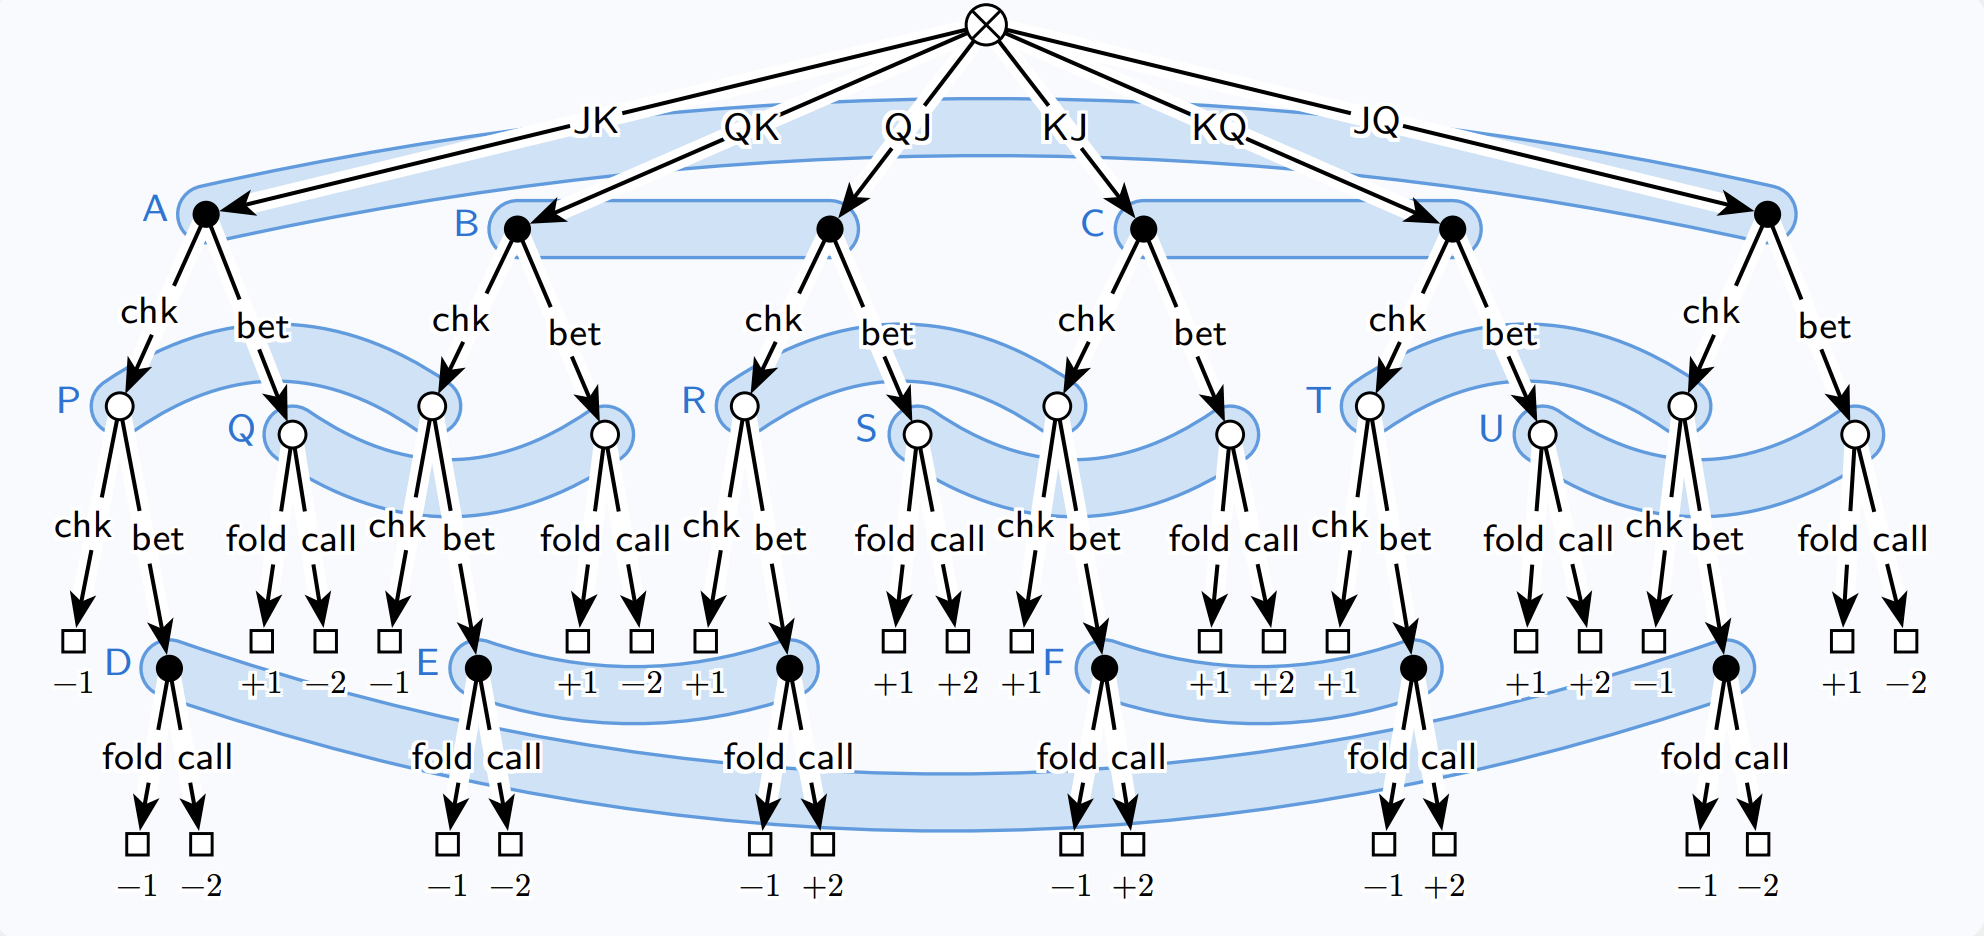
\includegraphics[scale=.44]{game_tree}
    \caption{Game tree of Kuhn Poker \cite{Farina}}
\end{figure}

\begin{center}
\textbf{Figure 2: strategy profile corresponding to computed Nash Equilibrium in Kuhn Poker}
\begin{tabular}{||c | c c c c||c | c c c c||}
\hline\hline

 \multicolumn{10}{||c||}{Strategy profile ($\sigma$)} \\
 
\hline\hline
 \multicolumn{5}{||c||}{P1 strategy profile ($\sigma_1$)} & 
 \multicolumn{5}{||c||}{P2 strategy profile ($\sigma_2$)} \\

 \hline
 Info Sets & Bet & Call & Check  & Fold &
 Info Sets & Bet & Call & Check  & Fold
 \\ [0.5ex] 
 \hline\hline
 J & 0.2010 & 0 & 0.7989 & 0 & 
 J.BET & 0 & 0.0005 & 0 & 0.9995\\ [1ex] 
 \hline
 Q & 0.0034 & 0 & 0.9965 & 1 & 
 Q.BET & 0 & 0.3687 & 0 & 0.6312\\ [1ex] 
 \hline
 K & 0.5984 & 0 & 0.4015 & 0 & 
 K.BET & 0 & 0.9995 & 0 & 0.0005\\ [1ex] 
 \hline
 J.CHECK.BET & 0 & 0.0003 & 0 & 0.9996 & 
 J.CHECK & 0.3276 & 0 & 0.6723 & 0\\ [1ex] 
 \hline
 Q.CHECK.BET & 0 & 0.5680 & 0 & 0.4319 & 
 Q.CHECK & 0.0037 & 0 & 0.9962 & 0\\ [1ex] 
 \hline
 K.CHECK.BET & 0 & 0.9993 & 0 & 0.0006 & 
 K.CHECK & 0.9995 & 0 & 0.0005 & 0\\ [1ex] 
 \hline
\end{tabular}
\end{center}
%%% LITTLE TABLES. 

\newpage


\begin{thebibliography}{9}

\bibitem{Zinkevich}
Martin A. Zinkevich, Michael Bradley Johanson, Michael Bowling, and Carmelo Piccione, \emph{Regret Minimization in Games with Incomplete Information}. Neural Information Processing Systems, 2007.

\bibitem{Wiedenbeck}
Bryce Wiedenbeck. \textit{Lecture 26: Counterfactual Regret Minimization (CFR)}. 
Davidson CSC 383: Algorithmic Game Theory, S23. 

\bibitem{Farina} Farina, G. (2024). \textit{Lecture 9: Extensive Form Games}. MIT 6.S890 - Topics in Multiagent Learning, Lecture 9.

\bibitem{Int8} Int8. (n.d.). \textit{Counterfactual Regret Minimization for Poker AI}.

\end{thebibliography}





\end{document}
